\documentclass[1p]{elsarticle_modified}
%\bibliographystyle{elsarticle-num}

%\usepackage[colorlinks]{hyperref}
%\usepackage{abbrmath_seonhwa} %\Abb, \Ascr, \Acal ,\Abf, \Afrak
\usepackage{amsfonts}
\usepackage{amssymb}
\usepackage{amsmath}
\usepackage{amsthm}
\usepackage{scalefnt}
\usepackage{amsbsy}
\usepackage{kotex}
\usepackage{caption}
\usepackage{subfig}
\usepackage{color}
\usepackage{graphicx}
\usepackage{xcolor} %% white, black, red, green, blue, cyan, magenta, yellow
\usepackage{float}
\usepackage{setspace}
\usepackage{hyperref}

\usepackage{tikz}
\usetikzlibrary{arrows}

\usepackage{multirow}
\usepackage{array} % fixed length table
\usepackage{hhline}

%%%%%%%%%%%%%%%%%%%%%
\makeatletter
\renewcommand*\env@matrix[1][\arraystretch]{%
	\edef\arraystretch{#1}%
	\hskip -\arraycolsep
	\let\@ifnextchar\new@ifnextchar
	\array{*\c@MaxMatrixCols c}}
\makeatother %https://tex.stackexchange.com/questions/14071/how-can-i-increase-the-line-spacing-in-a-matrix
%%%%%%%%%%%%%%%

\usepackage[normalem]{ulem}

\newcommand{\msout}[1]{\ifmmode\text{\sout{\ensuremath{#1}}}\else\sout{#1}\fi}
%SOURCE: \msout is \stkout macro in https://tex.stackexchange.com/questions/20609/strikeout-in-math-mode

\newcommand{\cancel}[1]{
	\ifmmode
	{\color{red}\msout{#1}}
	\else
	{\color{red}\sout{#1}}
	\fi
}

\newcommand{\add}[1]{
	{\color{blue}\uwave{#1}}
}

\newcommand{\replace}[2]{
	\ifmmode
	{\color{red}\msout{#1}}{\color{blue}\uwave{#2}}
	\else
	{\color{red}\sout{#1}}{\color{blue}\uwave{#2}}
	\fi
}

\newcommand{\Sol}{\mathcal{S}} %segment
\newcommand{\D}{D} %diagram
\newcommand{\A}{\mathcal{A}} %arc


%%%%%%%%%%%%%%%%%%%%%%%%%%%%%5 test

\def\sl{\operatorname{\textup{SL}}(2,\Cbb)}
\def\psl{\operatorname{\textup{PSL}}(2,\Cbb)}
\def\quan{\mkern 1mu \triangleright \mkern 1mu}

\theoremstyle{definition}
\newtheorem{thm}{Theorem}[section]
\newtheorem{prop}[thm]{Proposition}
\newtheorem{lem}[thm]{Lemma}
\newtheorem{ques}[thm]{Question}
\newtheorem{cor}[thm]{Corollary}
\newtheorem{defn}[thm]{Definition}
\newtheorem{exam}[thm]{Example}
\newtheorem{rmk}[thm]{Remark}
\newtheorem{alg}[thm]{Algorithm}

\newcommand{\I}{\sqrt{-1}}
\begin{document}

%\begin{frontmatter}
%
%\title{Boundary parabolic representations of knots up to 8 crossings}
%
%%% Group authors per affiliation:
%\author{Yunhi Cho} 
%\address{Department of Mathematics, University of Seoul, Seoul, Korea}
%\ead{yhcho@uos.ac.kr}
%
%
%\author{Seonhwa Kim} %\fnref{s_kim}}
%\address{Center for Geometry and Physics, Institute for Basic Science, Pohang, 37673, Korea}
%\ead{ryeona17@ibs.re.kr}
%
%\author{Hyuk Kim}
%\address{Department of Mathematical Sciences, Seoul National University, Seoul 08826, Korea}
%\ead{hyukkim@snu.ac.kr}
%
%\author{Seokbeom Yoon}
%\address{Department of Mathematical Sciences, Seoul National University, Seoul, 08826,  Korea}
%\ead{sbyoon15@snu.ac.kr}
%
%\begin{abstract}
%We find all boundary parabolic representation of knots up to 8 crossings.
%
%\end{abstract}
%\begin{keyword}
%    \MSC[2010] 57M25 
%\end{keyword}
%
%\end{frontmatter}

%\linenumbers
%\tableofcontents
%
\newcommand\colored[1]{\textcolor{white}{\rule[-0.35ex]{0.8em}{1.4ex}}\kern-0.8em\color{red} #1}%
%\newcommand\colored[1]{\textcolor{white}{ #1}\kern-2.17ex	\textcolor{white}{ #1}\kern-1.81ex	\textcolor{white}{ #1}\kern-2.15ex\color{red}#1	}

{\Large $\underline{12n_{0082}~(K12n_{0082})}$}

\setlength{\tabcolsep}{10pt}
\renewcommand{\arraystretch}{1.6}
\vspace{1cm}\begin{tabular}{m{100pt}>{\centering\arraybackslash}m{274pt}}
\multirow{5}{120pt}{
	\centering
	\includegraphics[width=112pt]{../../../GIT/diagram.site/Diagrams/png/2171_12n_0082.png}\\
\ \ \ A knot diagram\footnotemark}&
\allowdisplaybreaks
\textbf{Linearized knot diagam} \\
\cline{2-2}
 &
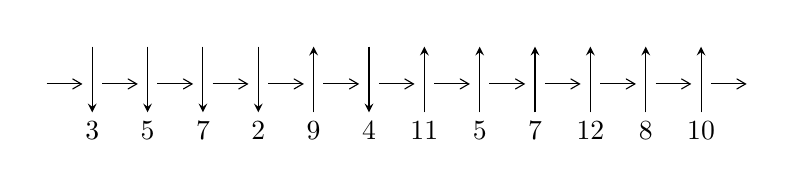
\begin{tikzpicture}[x=20pt, y=17pt]
	% nodes
	\node (C0) at (0, 0) {};
	\node (C1) at (1, 0) {};
	\node (C1U) at (1, +1) {};
	\node (C1D) at (1, -1) {3};

	\node (C2) at (2, 0) {};
	\node (C2U) at (2, +1) {};
	\node (C2D) at (2, -1) {5};

	\node (C3) at (3, 0) {};
	\node (C3U) at (3, +1) {};
	\node (C3D) at (3, -1) {7};

	\node (C4) at (4, 0) {};
	\node (C4U) at (4, +1) {};
	\node (C4D) at (4, -1) {2};

	\node (C5) at (5, 0) {};
	\node (C5U) at (5, +1) {};
	\node (C5D) at (5, -1) {9};

	\node (C6) at (6, 0) {};
	\node (C6U) at (6, +1) {};
	\node (C6D) at (6, -1) {4};

	\node (C7) at (7, 0) {};
	\node (C7U) at (7, +1) {};
	\node (C7D) at (7, -1) {11};

	\node (C8) at (8, 0) {};
	\node (C8U) at (8, +1) {};
	\node (C8D) at (8, -1) {5};

	\node (C9) at (9, 0) {};
	\node (C9U) at (9, +1) {};
	\node (C9D) at (9, -1) {7};

	\node (C10) at (10, 0) {};
	\node (C10U) at (10, +1) {};
	\node (C10D) at (10, -1) {12};

	\node (C11) at (11, 0) {};
	\node (C11U) at (11, +1) {};
	\node (C11D) at (11, -1) {8};

	\node (C12) at (12, 0) {};
	\node (C12U) at (12, +1) {};
	\node (C12D) at (12, -1) {10};
	\node (C13) at (13, 0) {};

	% arrows
	\draw[->,>={angle 60}]
	(C0) edge (C1) (C1) edge (C2) (C2) edge (C3) (C3) edge (C4) (C4) edge (C5) (C5) edge (C6) (C6) edge (C7) (C7) edge (C8) (C8) edge (C9) (C9) edge (C10) (C10) edge (C11) (C11) edge (C12) (C12) edge (C13) ;	\draw[->,>=stealth]
	(C1U) edge (C1D) (C2U) edge (C2D) (C3U) edge (C3D) (C4U) edge (C4D) (C5D) edge (C5U) (C6U) edge (C6D) (C7D) edge (C7U) (C8D) edge (C8U) (C9D) edge (C9U) (C10D) edge (C10U) (C11D) edge (C11U) (C12D) edge (C12U) ;
	\end{tikzpicture} \\
\hhline{~~} \\& 
\textbf{Solving Sequence} \\ \cline{2-2} 
 &
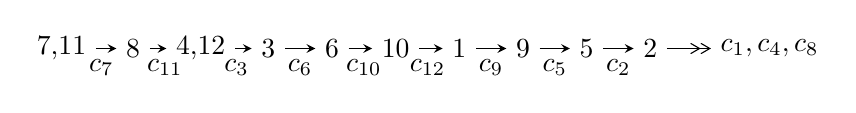
\begin{tikzpicture}[x=23pt, y=7pt]
	% node
	\node (A0) at (-1/8, 0) {7,11};
	\node (A1) at (1, 0) {8};
	\node (A2) at (33/16, 0) {4,12};
	\node (A3) at (25/8, 0) {3};
	\node (A4) at (33/8, 0) {6};
	\node (A5) at (41/8, 0) {10};
	\node (A6) at (49/8, 0) {1};
	\node (A7) at (57/8, 0) {9};
	\node (A8) at (65/8, 0) {5};
	\node (A9) at (73/8, 0) {2};
	\node (C1) at (1/2, -1) {$c_{7}$};
	\node (C2) at (3/2, -1) {$c_{11}$};
	\node (C3) at (21/8, -1) {$c_{3}$};
	\node (C4) at (29/8, -1) {$c_{6}$};
	\node (C5) at (37/8, -1) {$c_{10}$};
	\node (C6) at (45/8, -1) {$c_{12}$};
	\node (C7) at (53/8, -1) {$c_{9}$};
	\node (C8) at (61/8, -1) {$c_{5}$};
	\node (C9) at (69/8, -1) {$c_{2}$};
	\node (A10) at (11, 0) {$c_{1},c_{4},c_{8}$};

	% edge
	\draw[->,>=stealth]	
	(A0) edge (A1) (A1) edge (A2) (A2) edge (A3) (A3) edge (A4) (A4) edge (A5) (A5) edge (A6) (A6) edge (A7) (A7) edge (A8) (A8) edge (A9) ;
	\draw[->>,>={angle 60}]	
	(A9) edge (A10);
\end{tikzpicture} \\ 

\end{tabular} \\

\footnotetext{
The image of knot diagram is generated by the software ``\textbf{Draw programme}" developed by Andrew Bartholomew(\url{http://www.layer8.co.uk/maths/draw/index.htm\#Running-draw}), where we modified some parts for our purpose(\url{https://github.com/CATsTAILs/LinksPainter}).
}\phantom \\ \newline 
\centering \textbf{Ideals for irreducible components\footnotemark of $X_{\text{par}}$} 
 
\begin{align*}
I^u_{1}&=\langle 
-1075292995 u^{33}-4308557086 u^{32}+\cdots+1783382596 b-2108461367,\\
\phantom{I^u_{1}}&\phantom{= \langle  }-16834407501 u^{33}-77191989494 u^{32}+\cdots+1783382596 a-50354623549,\\
\phantom{I^u_{1}}&\phantom{= \langle  }u^{34}+5 u^{33}+\cdots+17 u+1\rangle \\
I^u_{2}&=\langle 
b,\;3 u^7+u^6-4 u^5-4 u^4+5 u^3+3 u^2+a- u-5,\;u^8+u^7- u^6-2 u^5+u^4+2 u^3-2 u-1\rangle \\
I^u_{3}&=\langle 
- u^2 a-2 u^2+b+a+u+2,\;a^2+2 a u+4 u^2+a-4 u+4,\;u^3- u^2+1\rangle \\
I^u_{4}&=\langle 
u^2+b,\;a- u,\;u^3- u^2+1\rangle \\
\\
\end{align*}
\raggedright * 4 irreducible components of $\dim_{\mathbb{C}}=0$, with total 51 representations.\\
\footnotetext{All coefficients of polynomials are rational numbers. But the coefficients are sometimes approximated in decimal forms when there is not enough margin.}
\newpage
\renewcommand{\arraystretch}{1}
\centering \section*{I. $I^u_{1}= \langle -1.08\times10^{9} u^{33}-4.31\times10^{9} u^{32}+\cdots+1.78\times10^{9} b-2.11\times10^{9},\;-1.68\times10^{10} u^{33}-7.72\times10^{10} u^{32}+\cdots+1.78\times10^{9} a-5.04\times10^{10},\;u^{34}+5 u^{33}+\cdots+17 u+1 \rangle$}
\flushleft \textbf{(i) Arc colorings}\\
\begin{tabular}{m{7pt} m{180pt} m{7pt} m{180pt} }
\flushright $a_{7}=$&$\begin{pmatrix}1\\0\end{pmatrix}$ \\
\flushright $a_{11}=$&$\begin{pmatrix}0\\u\end{pmatrix}$ \\
\flushright $a_{8}=$&$\begin{pmatrix}1\\- u^2\end{pmatrix}$ \\
\flushright $a_{4}=$&$\begin{pmatrix}9.43959 u^{33}+43.2840 u^{32}+\cdots+295.933 u+28.2355\\0.602951 u^{33}+2.41595 u^{32}+\cdots+10.5760 u+1.18228\end{pmatrix}$ \\
\flushright $a_{12}=$&$\begin{pmatrix}u\\- u^3+u\end{pmatrix}$ \\
\flushright $a_{3}=$&$\begin{pmatrix}10.0425 u^{33}+45.7000 u^{32}+\cdots+306.509 u+29.4177\\0.602951 u^{33}+2.41595 u^{32}+\cdots+10.5760 u+1.18228\end{pmatrix}$ \\
\flushright $a_{6}=$&$\begin{pmatrix}-8.32985 u^{33}-34.9914 u^{32}+\cdots-174.842 u-14.4784\\1.50407 u^{33}+6.20192 u^{32}+\cdots+28.1402 u+1.51861\end{pmatrix}$ \\
\flushright $a_{10}=$&$\begin{pmatrix}- u^3\\u^5- u^3+u\end{pmatrix}$ \\
\flushright $a_{1}=$&$\begin{pmatrix}u^5+u\\- u^7+u^5-2 u^3+u\end{pmatrix}$ \\
\flushright $a_{9}=$&$\begin{pmatrix}- u^5- u\\u^5- u^3+u\end{pmatrix}$ \\
\flushright $a_{5}=$&$\begin{pmatrix}-3.94864 u^{33}-16.6164 u^{32}+\cdots-92.4717 u-9.25517\\-0.647049 u^{33}-2.83405 u^{32}+\cdots-12.4240 u-1.06772\end{pmatrix}$ \\
\flushright $a_{2}=$&$\begin{pmatrix}7.18982 u^{33}+33.9328 u^{32}+\cdots+248.452 u+22.9281\\0.647049 u^{33}+2.83405 u^{32}+\cdots+12.4240 u+1.06772\end{pmatrix}$\\&\end{tabular}
\flushleft \textbf{(ii) Obstruction class $= -1$}\\~\\
\flushleft \textbf{(iii) Cusp Shapes $= -\frac{749238525}{445845649} u^{33}-\frac{25224574109}{1783382596} u^{32}+\cdots-\frac{515748589297}{1783382596} u-\frac{13447700611}{445845649}$}\\~\\
\newpage\renewcommand{\arraystretch}{1}
\flushleft \textbf{(iv) u-Polynomials at the component}\newline \\
\begin{tabular}{m{50pt}|m{274pt}}
Crossings & \hspace{64pt}u-Polynomials at each crossing \\
\hline $$\begin{aligned}c_{1}\end{aligned}$$&$\begin{aligned}
&u^{34}+40 u^{32}+\cdots+1011 u+1
\end{aligned}$\\
\hline $$\begin{aligned}c_{2},c_{4}\end{aligned}$$&$\begin{aligned}
&u^{34}-12 u^{33}+\cdots+27 u+1
\end{aligned}$\\
\hline $$\begin{aligned}c_{3},c_{6}\end{aligned}$$&$\begin{aligned}
&u^{34}-4 u^{33}+\cdots+896 u-256
\end{aligned}$\\
\hline $$\begin{aligned}c_{5},c_{8}\end{aligned}$$&$\begin{aligned}
&u^{34}-2 u^{33}+\cdots-1536 u-512
\end{aligned}$\\
\hline $$\begin{aligned}c_{7},c_{11}\end{aligned}$$&$\begin{aligned}
&u^{34}-5 u^{33}+\cdots-17 u+1
\end{aligned}$\\
\hline $$\begin{aligned}c_{9}\end{aligned}$$&$\begin{aligned}
&u^{34}+5 u^{33}+\cdots-34224 u+2116
\end{aligned}$\\
\hline $$\begin{aligned}c_{10},c_{12}\end{aligned}$$&$\begin{aligned}
&u^{34}-15 u^{33}+\cdots-147 u+1
\end{aligned}$\\
\hline
\end{tabular}\\~\\
\newpage\renewcommand{\arraystretch}{1}
\flushleft \textbf{(v) Riley Polynomials at the component}\newline \\
\begin{tabular}{m{50pt}|m{274pt}}
Crossings & \hspace{64pt}Riley Polynomials at each crossing \\
\hline $$\begin{aligned}c_{1}\end{aligned}$$&$\begin{aligned}
&y^{34}+80 y^{33}+\cdots-1049111 y+1
\end{aligned}$\\
\hline $$\begin{aligned}c_{2},c_{4}\end{aligned}$$&$\begin{aligned}
&y^{34}+40 y^{32}+\cdots-1011 y+1
\end{aligned}$\\
\hline $$\begin{aligned}c_{3},c_{6}\end{aligned}$$&$\begin{aligned}
&y^{34}+60 y^{33}+\cdots-2146304 y+65536
\end{aligned}$\\
\hline $$\begin{aligned}c_{5},c_{8}\end{aligned}$$&$\begin{aligned}
&y^{34}-56 y^{33}+\cdots-1441792 y+262144
\end{aligned}$\\
\hline $$\begin{aligned}c_{7},c_{11}\end{aligned}$$&$\begin{aligned}
&y^{34}-15 y^{33}+\cdots-147 y+1
\end{aligned}$\\
\hline $$\begin{aligned}c_{9}\end{aligned}$$&$\begin{aligned}
&y^{34}-83 y^{33}+\cdots-660094664 y+4477456
\end{aligned}$\\
\hline $$\begin{aligned}c_{10},c_{12}\end{aligned}$$&$\begin{aligned}
&y^{34}+13 y^{33}+\cdots-18915 y+1
\end{aligned}$\\
\hline
\end{tabular}\\~\\
\newpage\flushleft \textbf{(vi) Complex Volumes and Cusp Shapes}
$$\begin{array}{c|c|c}  
\text{Solutions to }I^u_{1}& \I (\text{vol} + \sqrt{-1}CS) & \text{Cusp shape}\\
 \hline 
\begin{aligned}
u &= -0.675479 + 0.712354 I \\
a &= -0.270719 + 0.161827 I \\
b &= \phantom{-}0.097932 - 0.857151 I\end{aligned}
 & \phantom{-}0.11560 + 2.14584 I & \phantom{-}4.84697 - 4.28283 I \\ \hline\begin{aligned}
u &= -0.675479 - 0.712354 I \\
a &= -0.270719 - 0.161827 I \\
b &= \phantom{-}0.097932 + 0.857151 I\end{aligned}
 & \phantom{-}0.11560 - 2.14584 I & \phantom{-}4.84697 + 4.28283 I \\ \hline\begin{aligned}
u &= \phantom{-}0.787838 + 0.675769 I \\
a &= -0.413189 + 0.782228 I \\
b &= \phantom{-}0.360422 - 0.507830 I\end{aligned}
 & -2.05683 + 2.19416 I & \phantom{-}2.78133 - 4.16804 I \\ \hline\begin{aligned}
u &= \phantom{-}0.787838 - 0.675769 I \\
a &= -0.413189 - 0.782228 I \\
b &= \phantom{-}0.360422 + 0.507830 I\end{aligned}
 & -2.05683 - 2.19416 I & \phantom{-}2.78133 + 4.16804 I \\ \hline\begin{aligned}
u &= -0.994788 + 0.364572 I \\
a &= -1.43728 - 0.32761 I \\
b &= \phantom{-}1.097360 - 0.422286 I\end{aligned}
 & \phantom{-}0.27995 - 2.43239 I & \phantom{-}4.42150 + 3.66524 I \\ \hline\begin{aligned}
u &= -0.994788 - 0.364572 I \\
a &= -1.43728 + 0.32761 I \\
b &= \phantom{-}1.097360 + 0.422286 I\end{aligned}
 & \phantom{-}0.27995 + 2.43239 I & \phantom{-}4.42150 - 3.66524 I \\ \hline\begin{aligned}
u &= \phantom{-}0.883198 + 0.167536 I \\
a &= -0.82822 - 2.77937 I \\
b &= \phantom{-}0.390635 + 1.309810 I\end{aligned}
 & \phantom{-}4.40661 - 2.39050 I & \phantom{-}8.72484 - 4.03068 I \\ \hline\begin{aligned}
u &= \phantom{-}0.883198 - 0.167536 I \\
a &= -0.82822 + 2.77937 I \\
b &= \phantom{-}0.390635 - 1.309810 I\end{aligned}
 & \phantom{-}4.40661 + 2.39050 I & \phantom{-}8.72484 + 4.03068 I \\ \hline\begin{aligned}
u &= -0.439134 + 1.012860 I \\
a &= -0.14054 + 2.08289 I \\
b &= -0.21712 - 2.33804 I\end{aligned}
 & \phantom{-}12.94380 - 1.52834 I & \phantom{-}2.89091 + 1.52951 I \\ \hline\begin{aligned}
u &= -0.439134 - 1.012860 I \\
a &= -0.14054 - 2.08289 I \\
b &= -0.21712 + 2.33804 I\end{aligned}
 & \phantom{-}12.94380 + 1.52834 I & \phantom{-}2.89091 - 1.52951 I\\
 \hline 
 \end{array}$$\newpage$$\begin{array}{c|c|c}  
\text{Solutions to }I^u_{1}& \I (\text{vol} + \sqrt{-1}CS) & \text{Cusp shape}\\
 \hline 
\begin{aligned}
u &= -0.554438 + 0.988490 I \\
a &= \phantom{-}0.37372 - 1.78363 I \\
b &= -0.69939 + 2.06047 I\end{aligned}
 & \phantom{-}12.1480 + 7.3055 I & \phantom{-}2.34511 - 2.34014 I \\ \hline\begin{aligned}
u &= -0.554438 - 0.988490 I \\
a &= \phantom{-}0.37372 + 1.78363 I \\
b &= -0.69939 - 2.06047 I\end{aligned}
 & \phantom{-}12.1480 - 7.3055 I & \phantom{-}2.34511 + 2.34014 I \\ \hline\begin{aligned}
u &= \phantom{-}0.877826 + 0.731952 I \\
a &= -2.89148 - 0.75774 I \\
b &= -0.433493 + 0.039285 I\end{aligned}
 & -4.30564 + 2.78916 I & -43.5792 - 1.9775 I \\ \hline\begin{aligned}
u &= \phantom{-}0.877826 - 0.731952 I \\
a &= -2.89148 + 0.75774 I \\
b &= -0.433493 - 0.039285 I\end{aligned}
 & -4.30564 - 2.78916 I & -43.5792 + 1.9775 I \\ \hline\begin{aligned}
u &= \phantom{-}0.960792 + 0.643718 I \\
a &= -1.56912 - 0.34499 I \\
b &= \phantom{-}0.705310 + 0.607713 I\end{aligned}
 & -1.51157 + 2.93275 I & \phantom{-}3.49597 - 2.09060 I \\ \hline\begin{aligned}
u &= \phantom{-}0.960792 - 0.643718 I \\
a &= -1.56912 + 0.34499 I \\
b &= \phantom{-}0.705310 - 0.607713 I\end{aligned}
 & -1.51157 - 2.93275 I & \phantom{-}3.49597 + 2.09060 I \\ \hline\begin{aligned}
u &= -0.988094 + 0.655947 I \\
a &= \phantom{-}0.798191 - 0.915301 I \\
b &= \phantom{-}0.242079 + 0.838628 I\end{aligned}
 & \phantom{-}1.06007 - 7.41163 I & \phantom{-}6.37706 + 10.12845 I \\ \hline\begin{aligned}
u &= -0.988094 - 0.655947 I \\
a &= \phantom{-}0.798191 + 0.915301 I \\
b &= \phantom{-}0.242079 - 0.838628 I\end{aligned}
 & \phantom{-}1.06007 + 7.41163 I & \phantom{-}6.37706 - 10.12845 I \\ \hline\begin{aligned}
u &= \phantom{-}1.134070 + 0.366301 I \\
a &= \phantom{-}1.64472 + 3.48212 I \\
b &= -0.39273 - 1.87590 I\end{aligned}
 & \phantom{-}6.17981 + 3.91713 I & \phantom{-}6.50133 - 4.05550 I \\ \hline\begin{aligned}
u &= \phantom{-}1.134070 - 0.366301 I \\
a &= \phantom{-}1.64472 - 3.48212 I \\
b &= -0.39273 + 1.87590 I\end{aligned}
 & \phantom{-}6.17981 - 3.91713 I & \phantom{-}6.50133 + 4.05550 I\\
 \hline 
 \end{array}$$\newpage$$\begin{array}{c|c|c}  
\text{Solutions to }I^u_{1}& \I (\text{vol} + \sqrt{-1}CS) & \text{Cusp shape}\\
 \hline 
\begin{aligned}
u &= -0.759460 + 0.212841 I \\
a &= \phantom{-}2.07551 - 3.57649 I \\
b &= \phantom{-}0.167778 + 0.535642 I\end{aligned}
 & -0.839427 - 0.307998 I & \phantom{-}10.22671 + 6.42071 I \\ \hline\begin{aligned}
u &= -0.759460 - 0.212841 I \\
a &= \phantom{-}2.07551 + 3.57649 I \\
b &= \phantom{-}0.167778 - 0.535642 I\end{aligned}
 & -0.839427 + 0.307998 I & \phantom{-}10.22671 - 6.42071 I \\ \hline\begin{aligned}
u &= -0.199261 + 0.726308 I \\
a &= \phantom{-}0.009119 - 0.678462 I \\
b &= -0.695938 + 1.120220 I\end{aligned}
 & \phantom{-}2.39265 - 0.51912 I & \phantom{-}3.37017 + 1.09835 I \\ \hline\begin{aligned}
u &= -0.199261 - 0.726308 I \\
a &= \phantom{-}0.009119 + 0.678462 I \\
b &= -0.695938 - 1.120220 I\end{aligned}
 & \phantom{-}2.39265 + 0.51912 I & \phantom{-}3.37017 - 1.09835 I \\ \hline\begin{aligned}
u &= -1.155100 + 0.509124 I \\
a &= \phantom{-}0.68550 + 3.05854 I \\
b &= -1.31414 - 1.23344 I\end{aligned}
 & \phantom{-}5.17110 - 4.13601 I & \phantom{-}6.26603 + 3.46699 I \\ \hline\begin{aligned}
u &= -1.155100 - 0.509124 I \\
a &= \phantom{-}0.68550 - 3.05854 I \\
b &= -1.31414 + 1.23344 I\end{aligned}
 & \phantom{-}5.17110 + 4.13601 I & \phantom{-}6.26603 - 3.46699 I \\ \hline\begin{aligned}
u &= \phantom{-}1.331470 + 0.064618 I \\
a &= \phantom{-}0.73597 - 5.01515 I \\
b &= -0.62913 + 2.45336 I\end{aligned}
 & \phantom{-}19.5904 + 4.8180 I & \phantom{-}6.85242 - 2.12746 I \\ \hline\begin{aligned}
u &= \phantom{-}1.331470 - 0.064618 I \\
a &= \phantom{-}0.73597 + 5.01515 I \\
b &= -0.62913 - 2.45336 I\end{aligned}
 & \phantom{-}19.5904 - 4.8180 I & \phantom{-}6.85242 + 2.12746 I \\ \hline\begin{aligned}
u &= -0.647070\phantom{ +0.000000I} \\
a &= -0.602677\phantom{ +0.000000I} \\
b &= -0.176681\phantom{ +0.000000I}\end{aligned}
 & \phantom{-}0.883121\phantom{ +0.000000I} & \phantom{-}11.7300\phantom{ +0.000000I} \\ \hline\begin{aligned}
u &= -1.141270 + 0.734626 I \\
a &= -1.07593 + 3.44611 I \\
b &= -0.83809 - 1.99730 I\end{aligned}
 & \phantom{-}13.9751 - 13.5871 I & \phantom{-}3.82321 + 6.38940 I\\
 \hline 
 \end{array}$$\newpage$$\begin{array}{c|c|c}  
\text{Solutions to }I^u_{1}& \I (\text{vol} + \sqrt{-1}CS) & \text{Cusp shape}\\
 \hline 
\begin{aligned}
u &= -1.141270 - 0.734626 I \\
a &= -1.07593 - 3.44611 I \\
b &= -0.83809 + 1.99730 I\end{aligned}
 & \phantom{-}13.9751 + 13.5871 I & \phantom{-}3.82321 - 6.38940 I \\ \hline\begin{aligned}
u &= -1.202000 + 0.684331 I \\
a &= \phantom{-}1.86014 - 3.56344 I \\
b &= \phantom{-}0.00069 + 2.47834 I\end{aligned}
 & \phantom{-}15.3278 - 4.6468 I & \phantom{-}5.01393 + 2.36080 I \\ \hline\begin{aligned}
u &= -1.202000 - 0.684331 I \\
a &= \phantom{-}1.86014 + 3.56344 I \\
b &= \phantom{-}0.00069 - 2.47834 I\end{aligned}
 & \phantom{-}15.3278 + 4.6468 I & \phantom{-}5.01393 - 2.36080 I \\ \hline\begin{aligned}
u &= -0.0852780\phantom{ +0.000000I} \\
a &= \phantom{-}8.48988\phantom{ +0.000000I} \\
b &= \phantom{-}0.492352\phantom{ +0.000000I}\end{aligned}
 & -1.21008\phantom{ +0.000000I} & -9.44660\phantom{ +0.000000I}\\
 \hline 
 \end{array}$$\newpage\newpage\renewcommand{\arraystretch}{1}
\centering \section*{II. $I^u_{2}= \langle b,\;3 u^7+u^6-4 u^5-4 u^4+5 u^3+3 u^2+a- u-5,\;u^8+u^7- u^6-2 u^5+u^4+2 u^3-2 u-1 \rangle$}
\flushleft \textbf{(i) Arc colorings}\\
\begin{tabular}{m{7pt} m{180pt} m{7pt} m{180pt} }
\flushright $a_{7}=$&$\begin{pmatrix}1\\0\end{pmatrix}$ \\
\flushright $a_{11}=$&$\begin{pmatrix}0\\u\end{pmatrix}$ \\
\flushright $a_{8}=$&$\begin{pmatrix}1\\- u^2\end{pmatrix}$ \\
\flushright $a_{4}=$&$\begin{pmatrix}-3 u^7- u^6+4 u^5+4 u^4-5 u^3-3 u^2+u+5\\0\end{pmatrix}$ \\
\flushright $a_{12}=$&$\begin{pmatrix}u\\- u^3+u\end{pmatrix}$ \\
\flushright $a_{3}=$&$\begin{pmatrix}-3 u^7- u^6+4 u^5+4 u^4-5 u^3-3 u^2+u+5\\0\end{pmatrix}$ \\
\flushright $a_{6}=$&$\begin{pmatrix}1\\0\end{pmatrix}$ \\
\flushright $a_{10}=$&$\begin{pmatrix}- u^3\\u^5- u^3+u\end{pmatrix}$ \\
\flushright $a_{1}=$&$\begin{pmatrix}u^5+u\\- u^7+u^5-2 u^3+u\end{pmatrix}$ \\
\flushright $a_{9}=$&$\begin{pmatrix}- u^5- u\\u^5- u^3+u\end{pmatrix}$ \\
\flushright $a_{5}=$&$\begin{pmatrix}- u^5- u\\u^7- u^5+2 u^3- u\end{pmatrix}$ \\
\flushright $a_{2}=$&$\begin{pmatrix}-3 u^7- u^6+5 u^5+4 u^4-5 u^3-3 u^2+2 u+5\\- u^7+u^5-2 u^3+u\end{pmatrix}$\\&\end{tabular}
\flushleft \textbf{(ii) Obstruction class $= 1$}\\~\\
\flushleft \textbf{(iii) Cusp Shapes $= -17 u^7-6 u^6+24 u^5+22 u^4-31 u^3-17 u^2+12 u+31$}\\~\\
\newpage\renewcommand{\arraystretch}{1}
\flushleft \textbf{(iv) u-Polynomials at the component}\newline \\
\begin{tabular}{m{50pt}|m{274pt}}
Crossings & \hspace{64pt}u-Polynomials at each crossing \\
\hline $$\begin{aligned}c_{1},c_{2}\end{aligned}$$&$\begin{aligned}
&(u-1)^8
\end{aligned}$\\
\hline $$\begin{aligned}c_{3},c_{6}\end{aligned}$$&$\begin{aligned}
&u^8
\end{aligned}$\\
\hline $$\begin{aligned}c_{4}\end{aligned}$$&$\begin{aligned}
&(u+1)^8
\end{aligned}$\\
\hline $$\begin{aligned}c_{5}\end{aligned}$$&$\begin{aligned}
&u^8- u^7-3 u^6+2 u^5+3 u^4-2 u-1
\end{aligned}$\\
\hline $$\begin{aligned}c_{7}\end{aligned}$$&$\begin{aligned}
&u^8+u^7- u^6-2 u^5+u^4+2 u^3-2 u-1
\end{aligned}$\\
\hline $$\begin{aligned}c_{8},c_{9}\end{aligned}$$&$\begin{aligned}
&u^8+u^7-3 u^6-2 u^5+3 u^4+2 u-1
\end{aligned}$\\
\hline $$\begin{aligned}c_{10}\end{aligned}$$&$\begin{aligned}
&u^8+3 u^7+7 u^6+10 u^5+11 u^4+10 u^3+6 u^2+4 u+1
\end{aligned}$\\
\hline $$\begin{aligned}c_{11}\end{aligned}$$&$\begin{aligned}
&u^8- u^7- u^6+2 u^5+u^4-2 u^3+2 u-1
\end{aligned}$\\
\hline $$\begin{aligned}c_{12}\end{aligned}$$&$\begin{aligned}
&u^8-3 u^7+7 u^6-10 u^5+11 u^4-10 u^3+6 u^2-4 u+1
\end{aligned}$\\
\hline
\end{tabular}\\~\\
\newpage\renewcommand{\arraystretch}{1}
\flushleft \textbf{(v) Riley Polynomials at the component}\newline \\
\begin{tabular}{m{50pt}|m{274pt}}
Crossings & \hspace{64pt}Riley Polynomials at each crossing \\
\hline $$\begin{aligned}c_{1},c_{2},c_{4}\end{aligned}$$&$\begin{aligned}
&(y-1)^8
\end{aligned}$\\
\hline $$\begin{aligned}c_{3},c_{6}\end{aligned}$$&$\begin{aligned}
&y^8
\end{aligned}$\\
\hline $$\begin{aligned}c_{5},c_{8},c_{9}\end{aligned}$$&$\begin{aligned}
&y^8-7 y^7+19 y^6-22 y^5+3 y^4+14 y^3-6 y^2-4 y+1
\end{aligned}$\\
\hline $$\begin{aligned}c_{7},c_{11}\end{aligned}$$&$\begin{aligned}
&y^8-3 y^7+7 y^6-10 y^5+11 y^4-10 y^3+6 y^2-4 y+1
\end{aligned}$\\
\hline $$\begin{aligned}c_{10},c_{12}\end{aligned}$$&$\begin{aligned}
&y^8+5 y^7+11 y^6+6 y^5-17 y^4-34 y^3-22 y^2-4 y+1
\end{aligned}$\\
\hline
\end{tabular}\\~\\
\newpage\flushleft \textbf{(vi) Complex Volumes and Cusp Shapes}
$$\begin{array}{c|c|c}  
\text{Solutions to }I^u_{2}& \I (\text{vol} + \sqrt{-1}CS) & \text{Cusp shape}\\
 \hline 
\begin{aligned}
u &= -0.570868 + 0.730671 I \\
a &= \phantom{-}0.615431 - 0.295452 I \\
b &= \phantom{-0.000000 } 0\end{aligned}
 & -0.604279 + 1.131230 I & \phantom{-}1.048604 + 0.799861 I \\ \hline\begin{aligned}
u &= -0.570868 - 0.730671 I \\
a &= \phantom{-}0.615431 + 0.295452 I \\
b &= \phantom{-0.000000 } 0\end{aligned}
 & -0.604279 - 1.131230 I & \phantom{-}1.048604 - 0.799861 I \\ \hline\begin{aligned}
u &= \phantom{-}0.855237 + 0.665892 I \\
a &= -1.68119 - 0.49658 I \\
b &= \phantom{-0.000000 } 0\end{aligned}
 & -3.80435 + 2.57849 I & -0.86993 - 2.07507 I \\ \hline\begin{aligned}
u &= \phantom{-}0.855237 - 0.665892 I \\
a &= -1.68119 + 0.49658 I \\
b &= \phantom{-0.000000 } 0\end{aligned}
 & -3.80435 - 2.57849 I & -0.86993 + 2.07507 I \\ \hline\begin{aligned}
u &= \phantom{-}1.09818\phantom{ +0.000000I} \\
a &= \phantom{-}0.532015\phantom{ +0.000000I} \\
b &= \phantom{-0.000000 } 0\end{aligned}
 & \phantom{-}4.85780\phantom{ +0.000000I} & \phantom{-}9.68010\phantom{ +0.000000I} \\ \hline\begin{aligned}
u &= -1.031810 + 0.655470 I \\
a &= \phantom{-}0.473764 + 0.240160 I \\
b &= \phantom{-0.000000 } 0\end{aligned}
 & \phantom{-}0.73474 - 6.44354 I & \phantom{-}3.69048 + 2.66284 I \\ \hline\begin{aligned}
u &= -1.031810 - 0.655470 I \\
a &= \phantom{-}0.473764 - 0.240160 I \\
b &= \phantom{-0.000000 } 0\end{aligned}
 & \phantom{-}0.73474 + 6.44354 I & \phantom{-}3.69048 - 2.66284 I \\ \hline\begin{aligned}
u &= -0.603304\phantom{ +0.000000I} \\
a &= \phantom{-}4.65198\phantom{ +0.000000I} \\
b &= \phantom{-0.000000 } 0\end{aligned}
 & -0.799899\phantom{ +0.000000I} & \phantom{-}25.5820\phantom{ +0.000000I}\\
 \hline 
 \end{array}$$\newpage\newpage\renewcommand{\arraystretch}{1}
\centering \section*{III. $I^u_{3}= \langle - u^2 a-2 u^2+b+a+u+2,\;a^2+2 a u+4 u^2+a-4 u+4,\;u^3- u^2+1 \rangle$}
\flushleft \textbf{(i) Arc colorings}\\
\begin{tabular}{m{7pt} m{180pt} m{7pt} m{180pt} }
\flushright $a_{7}=$&$\begin{pmatrix}1\\0\end{pmatrix}$ \\
\flushright $a_{11}=$&$\begin{pmatrix}0\\u\end{pmatrix}$ \\
\flushright $a_{8}=$&$\begin{pmatrix}1\\- u^2\end{pmatrix}$ \\
\flushright $a_{4}=$&$\begin{pmatrix}a\\u^2 a+2 u^2- a- u-2\end{pmatrix}$ \\
\flushright $a_{12}=$&$\begin{pmatrix}u\\- u^2+u+1\end{pmatrix}$ \\
\flushright $a_{3}=$&$\begin{pmatrix}u^2 a+2 u^2- u-2\\u^2 a+2 u^2- a- u-2\end{pmatrix}$ \\
\flushright $a_{6}=$&$\begin{pmatrix}u^2 a- a u- a-3\\u^2 a+a u+3 u^2\end{pmatrix}$ \\
\flushright $a_{10}=$&$\begin{pmatrix}- u^2+1\\- u^2\end{pmatrix}$ \\
\flushright $a_{1}=$&$\begin{pmatrix}-1\\0\end{pmatrix}$ \\
\flushright $a_{9}=$&$\begin{pmatrix}1\\- u^2\end{pmatrix}$ \\
\flushright $a_{5}=$&$\begin{pmatrix}u^2 a- a u- a-3\\u^2 a+a u+3 u^2\end{pmatrix}$ \\
\flushright $a_{2}=$&$\begin{pmatrix}2 u^2 a+3 u^2- a-5\\u^2 a+a u+3 u^2\end{pmatrix}$\\&\end{tabular}
\flushleft \textbf{(ii) Obstruction class $= 1$}\\~\\
\flushleft \textbf{(iii) Cusp Shapes $= u^2 a-7 a u-12 u^2-3 a-4 u+4$}\\~\\
\newpage\renewcommand{\arraystretch}{1}
\flushleft \textbf{(iv) u-Polynomials at the component}\newline \\
\begin{tabular}{m{50pt}|m{274pt}}
Crossings & \hspace{64pt}u-Polynomials at each crossing \\
\hline $$\begin{aligned}c_{1},c_{3},c_{9}\\c_{12}\end{aligned}$$&$\begin{aligned}
&(u^3- u^2+2 u-1)^2
\end{aligned}$\\
\hline $$\begin{aligned}c_{2},c_{11}\end{aligned}$$&$\begin{aligned}
&(u^3+u^2-1)^2
\end{aligned}$\\
\hline $$\begin{aligned}c_{4},c_{7}\end{aligned}$$&$\begin{aligned}
&(u^3- u^2+1)^2
\end{aligned}$\\
\hline $$\begin{aligned}c_{5},c_{8}\end{aligned}$$&$\begin{aligned}
&u^6
\end{aligned}$\\
\hline $$\begin{aligned}c_{6},c_{10}\end{aligned}$$&$\begin{aligned}
&(u^3+u^2+2 u+1)^2
\end{aligned}$\\
\hline
\end{tabular}\\~\\
\newpage\renewcommand{\arraystretch}{1}
\flushleft \textbf{(v) Riley Polynomials at the component}\newline \\
\begin{tabular}{m{50pt}|m{274pt}}
Crossings & \hspace{64pt}Riley Polynomials at each crossing \\
\hline $$\begin{aligned}c_{1},c_{3},c_{6}\\c_{9},c_{10},c_{12}\end{aligned}$$&$\begin{aligned}
&(y^3+3 y^2+2 y-1)^2
\end{aligned}$\\
\hline $$\begin{aligned}c_{2},c_{4},c_{7}\\c_{11}\end{aligned}$$&$\begin{aligned}
&(y^3- y^2+2 y-1)^2
\end{aligned}$\\
\hline $$\begin{aligned}c_{5},c_{8}\end{aligned}$$&$\begin{aligned}
&y^6
\end{aligned}$\\
\hline
\end{tabular}\\~\\
\newpage\flushleft \textbf{(vi) Complex Volumes and Cusp Shapes}
$$\begin{array}{c|c|c}  
\text{Solutions to }I^u_{3}& \I (\text{vol} + \sqrt{-1}CS) & \text{Cusp shape}\\
 \hline 
\begin{aligned}
u &= \phantom{-}0.877439 + 0.744862 I \\
a &= -1.06984 - 1.06527 I \\
b &= -0.215080 + 1.307140 I\end{aligned}
 & \phantom{-0.000000 -}5.65624 I & \phantom{-}3.29784 - 4.97572 I \\ \hline\begin{aligned}
u &= \phantom{-}0.877439 + 0.744862 I \\
a &= -1.68504 - 0.42445 I \\
b &= -0.569840\phantom{ +0.000000I}\end{aligned}
 & -4.13758 + 2.82812 I & \phantom{-}11.29331 - 8.29280 I \\ \hline\begin{aligned}
u &= \phantom{-}0.877439 - 0.744862 I \\
a &= -1.06984 + 1.06527 I \\
b &= -0.215080 - 1.307140 I\end{aligned}
 & \phantom{-0.000000 } -5.65624 I & \phantom{-}3.29784 + 4.97572 I \\ \hline\begin{aligned}
u &= \phantom{-}0.877439 - 0.744862 I \\
a &= -1.68504 + 0.42445 I \\
b &= -0.569840\phantom{ +0.000000I}\end{aligned}
 & -4.13758 - 2.82812 I & \phantom{-}11.29331 + 8.29280 I \\ \hline\begin{aligned}
u &= -0.754878\phantom{ +0.000000I} \\
a &= \phantom{-}0.25488 + 3.03873 I \\
b &= -0.215080 - 1.307140 I\end{aligned}
 & \phantom{-}4.13758 - 2.82812 I & \phantom{-}0.90884 + 8.67250 I \\ \hline\begin{aligned}
u &= -0.754878\phantom{ +0.000000I} \\
a &= \phantom{-}0.25488 - 3.03873 I \\
b &= -0.215080 + 1.307140 I\end{aligned}
 & \phantom{-}4.13758 + 2.82812 I & \phantom{-}0.90884 - 8.67250 I\\
 \hline 
 \end{array}$$\newpage\newpage\renewcommand{\arraystretch}{1}
\centering \section*{IV. $I^u_{4}= \langle u^2+b,\;a- u,\;u^3- u^2+1 \rangle$}
\flushleft \textbf{(i) Arc colorings}\\
\begin{tabular}{m{7pt} m{180pt} m{7pt} m{180pt} }
\flushright $a_{7}=$&$\begin{pmatrix}1\\0\end{pmatrix}$ \\
\flushright $a_{11}=$&$\begin{pmatrix}0\\u\end{pmatrix}$ \\
\flushright $a_{8}=$&$\begin{pmatrix}1\\- u^2\end{pmatrix}$ \\
\flushright $a_{4}=$&$\begin{pmatrix}u\\- u^2\end{pmatrix}$ \\
\flushright $a_{12}=$&$\begin{pmatrix}u\\- u^2+u+1\end{pmatrix}$ \\
\flushright $a_{3}=$&$\begin{pmatrix}- u^2+u\\- u^2\end{pmatrix}$ \\
\flushright $a_{6}=$&$\begin{pmatrix}u^2\\- u^2+u+1\end{pmatrix}$ \\
\flushright $a_{10}=$&$\begin{pmatrix}- u^2+1\\- u^2\end{pmatrix}$ \\
\flushright $a_{1}=$&$\begin{pmatrix}-1\\0\end{pmatrix}$ \\
\flushright $a_{9}=$&$\begin{pmatrix}1\\- u^2\end{pmatrix}$ \\
\flushright $a_{5}=$&$\begin{pmatrix}u^2\\- u^2+u+1\end{pmatrix}$ \\
\flushright $a_{2}=$&$\begin{pmatrix}u-1\\- u^2+u+1\end{pmatrix}$\\&\end{tabular}
\flushleft \textbf{(ii) Obstruction class $= 1$}\\~\\
\flushleft \textbf{(iii) Cusp Shapes $= -2 u^2+3 u+2$}\\~\\
\newpage\renewcommand{\arraystretch}{1}
\flushleft \textbf{(iv) u-Polynomials at the component}\newline \\
\begin{tabular}{m{50pt}|m{274pt}}
Crossings & \hspace{64pt}u-Polynomials at each crossing \\
\hline $$\begin{aligned}c_{1},c_{3},c_{9}\\c_{12}\end{aligned}$$&$\begin{aligned}
&u^3- u^2+2 u-1
\end{aligned}$\\
\hline $$\begin{aligned}c_{2},c_{11}\end{aligned}$$&$\begin{aligned}
&u^3+u^2-1
\end{aligned}$\\
\hline $$\begin{aligned}c_{4},c_{7}\end{aligned}$$&$\begin{aligned}
&u^3- u^2+1
\end{aligned}$\\
\hline $$\begin{aligned}c_{5},c_{8}\end{aligned}$$&$\begin{aligned}
&u^3
\end{aligned}$\\
\hline $$\begin{aligned}c_{6},c_{10}\end{aligned}$$&$\begin{aligned}
&u^3+u^2+2 u+1
\end{aligned}$\\
\hline
\end{tabular}\\~\\
\newpage\renewcommand{\arraystretch}{1}
\flushleft \textbf{(v) Riley Polynomials at the component}\newline \\
\begin{tabular}{m{50pt}|m{274pt}}
Crossings & \hspace{64pt}Riley Polynomials at each crossing \\
\hline $$\begin{aligned}c_{1},c_{3},c_{6}\\c_{9},c_{10},c_{12}\end{aligned}$$&$\begin{aligned}
&y^3+3 y^2+2 y-1
\end{aligned}$\\
\hline $$\begin{aligned}c_{2},c_{4},c_{7}\\c_{11}\end{aligned}$$&$\begin{aligned}
&y^3- y^2+2 y-1
\end{aligned}$\\
\hline $$\begin{aligned}c_{5},c_{8}\end{aligned}$$&$\begin{aligned}
&y^3
\end{aligned}$\\
\hline
\end{tabular}\\~\\
\newpage\flushleft \textbf{(vi) Complex Volumes and Cusp Shapes}
$$\begin{array}{c|c|c}  
\text{Solutions to }I^u_{4}& \I (\text{vol} + \sqrt{-1}CS) & \text{Cusp shape}\\
 \hline 
\begin{aligned}
u &= \phantom{-}0.877439 + 0.744862 I \\
a &= \phantom{-}0.877439 + 0.744862 I \\
b &= -0.215080 - 1.307140 I\end{aligned}
 & \phantom{-0.000000 } 0 & \phantom{-}4.20216 - 0.37970 I \\ \hline\begin{aligned}
u &= \phantom{-}0.877439 - 0.744862 I \\
a &= \phantom{-}0.877439 - 0.744862 I \\
b &= -0.215080 + 1.307140 I\end{aligned}
 & \phantom{-0.000000 } 0 & \phantom{-}4.20216 + 0.37970 I \\ \hline\begin{aligned}
u &= -0.754878\phantom{ +0.000000I} \\
a &= -0.754878\phantom{ +0.000000I} \\
b &= -0.569840\phantom{ +0.000000I}\end{aligned}
 & \phantom{-0.000000 } 0 & -1.40430\phantom{ +0.000000I}\\
 \hline 
 \end{array}$$\newpage
\newpage\renewcommand{\arraystretch}{1}
\centering \section*{ V. u-Polynomials}
\begin{tabular}{m{50pt}|m{274pt}}
Crossings & \hspace{64pt}u-Polynomials at each crossing \\
\hline $$\begin{aligned}c_{1}\end{aligned}$$&$\begin{aligned}
&((u-1)^8)(u^3- u^2+2 u-1)^3(u^{34}+40 u^{32}+\cdots+1011 u+1)
\end{aligned}$\\
\hline $$\begin{aligned}c_{2}\end{aligned}$$&$\begin{aligned}
&((u-1)^8)(u^3+u^2-1)^3(u^{34}-12 u^{33}+\cdots+27 u+1)
\end{aligned}$\\
\hline $$\begin{aligned}c_{3}\end{aligned}$$&$\begin{aligned}
&u^8(u^3- u^2+2 u-1)^3(u^{34}-4 u^{33}+\cdots+896 u-256)
\end{aligned}$\\
\hline $$\begin{aligned}c_{4}\end{aligned}$$&$\begin{aligned}
&((u+1)^8)(u^3- u^2+1)^3(u^{34}-12 u^{33}+\cdots+27 u+1)
\end{aligned}$\\
\hline $$\begin{aligned}c_{5}\end{aligned}$$&$\begin{aligned}
&u^9(u^8- u^7+\cdots-2 u-1)(u^{34}-2 u^{33}+\cdots-1536 u-512)
\end{aligned}$\\
\hline $$\begin{aligned}c_{6}\end{aligned}$$&$\begin{aligned}
&u^8(u^3+u^2+2 u+1)^3(u^{34}-4 u^{33}+\cdots+896 u-256)
\end{aligned}$\\
\hline $$\begin{aligned}c_{7}\end{aligned}$$&$\begin{aligned}
&(u^3- u^2+1)^3(u^8+u^7- u^6-2 u^5+u^4+2 u^3-2 u-1)\\
&\cdot(u^{34}-5 u^{33}+\cdots-17 u+1)
\end{aligned}$\\
\hline $$\begin{aligned}c_{8}\end{aligned}$$&$\begin{aligned}
&u^9(u^8+u^7+\cdots+2 u-1)(u^{34}-2 u^{33}+\cdots-1536 u-512)
\end{aligned}$\\
\hline $$\begin{aligned}c_{9}\end{aligned}$$&$\begin{aligned}
&(u^3- u^2+2 u-1)^3(u^8+u^7-3 u^6-2 u^5+3 u^4+2 u-1)\\
&\cdot(u^{34}+5 u^{33}+\cdots-34224 u+2116)
\end{aligned}$\\
\hline $$\begin{aligned}c_{10}\end{aligned}$$&$\begin{aligned}
&(u^3+u^2+2 u+1)^3\\
&\cdot(u^8+3 u^7+7 u^6+10 u^5+11 u^4+10 u^3+6 u^2+4 u+1)\\
&\cdot(u^{34}-15 u^{33}+\cdots-147 u+1)
\end{aligned}$\\
\hline $$\begin{aligned}c_{11}\end{aligned}$$&$\begin{aligned}
&(u^3+u^2-1)^3(u^8- u^7- u^6+2 u^5+u^4-2 u^3+2 u-1)\\
&\cdot(u^{34}-5 u^{33}+\cdots-17 u+1)
\end{aligned}$\\
\hline $$\begin{aligned}c_{12}\end{aligned}$$&$\begin{aligned}
&(u^3- u^2+2 u-1)^3\\
&\cdot(u^8-3 u^7+7 u^6-10 u^5+11 u^4-10 u^3+6 u^2-4 u+1)\\
&\cdot(u^{34}-15 u^{33}+\cdots-147 u+1)
\end{aligned}$\\
\hline
\end{tabular}\newpage\renewcommand{\arraystretch}{1}
\centering \section*{ VI. Riley Polynomials}
\begin{tabular}{m{50pt}|m{274pt}}
Crossings & \hspace{64pt}Riley Polynomials at each crossing \\
\hline $$\begin{aligned}c_{1}\end{aligned}$$&$\begin{aligned}
&((y-1)^8)(y^3+3 y^2+2 y-1)^3(y^{34}+80 y^{33}+\cdots-1049111 y+1)
\end{aligned}$\\
\hline $$\begin{aligned}c_{2},c_{4}\end{aligned}$$&$\begin{aligned}
&((y-1)^8)(y^3- y^2+2 y-1)^3(y^{34}+40 y^{32}+\cdots-1011 y+1)
\end{aligned}$\\
\hline $$\begin{aligned}c_{3},c_{6}\end{aligned}$$&$\begin{aligned}
&y^8(y^3+3 y^2+2 y-1)^3(y^{34}+60 y^{33}+\cdots-2146304 y+65536)
\end{aligned}$\\
\hline $$\begin{aligned}c_{5},c_{8}\end{aligned}$$&$\begin{aligned}
&y^9(y^8-7 y^7+19 y^6-22 y^5+3 y^4+14 y^3-6 y^2-4 y+1)\\
&\cdot(y^{34}-56 y^{33}+\cdots-1441792 y+262144)
\end{aligned}$\\
\hline $$\begin{aligned}c_{7},c_{11}\end{aligned}$$&$\begin{aligned}
&(y^3- y^2+2 y-1)^3\\
&\cdot(y^8-3 y^7+7 y^6-10 y^5+11 y^4-10 y^3+6 y^2-4 y+1)\\
&\cdot(y^{34}-15 y^{33}+\cdots-147 y+1)
\end{aligned}$\\
\hline $$\begin{aligned}c_{9}\end{aligned}$$&$\begin{aligned}
&(y^3+3 y^2+2 y-1)^3\\
&\cdot(y^8-7 y^7+19 y^6-22 y^5+3 y^4+14 y^3-6 y^2-4 y+1)\\
&\cdot(y^{34}-83 y^{33}+\cdots-660094664 y+4477456)
\end{aligned}$\\
\hline $$\begin{aligned}c_{10},c_{12}\end{aligned}$$&$\begin{aligned}
&(y^3+3 y^2+2 y-1)^3\\
&\cdot(y^8+5 y^7+11 y^6+6 y^5-17 y^4-34 y^3-22 y^2-4 y+1)\\
&\cdot(y^{34}+13 y^{33}+\cdots-18915 y+1)
\end{aligned}$\\
\hline
\end{tabular}
\vskip 2pc
\end{document}